
% \title[Adjoint-based design optimisation] {Adjoint-based design
%   optimisation for steady and unsteady flows}
% \author[J.-D. M\"{u}ller]%
% {J.-D. M\"{u}ller \\
%   {\small Queen Mary, University of London}\\[10pt]
%   collaborators:\\
%   D.~Jones, S.~Xu, F.~Christakpoulos, W.~Jahn, M.~Oriani%, {\small QMUL}%
% %\\S.~Bayyuk, V.~Brown, {\small ESI} 
% }
% 
% \date{Imperial College, London,\\ 28 June 2013}




% Handcrafted title-page.
\setbeamertemplate{background canvas}{%
%  \begin{center}
%    \includegraphics[width=\textwidth]{flowfield}\\
%    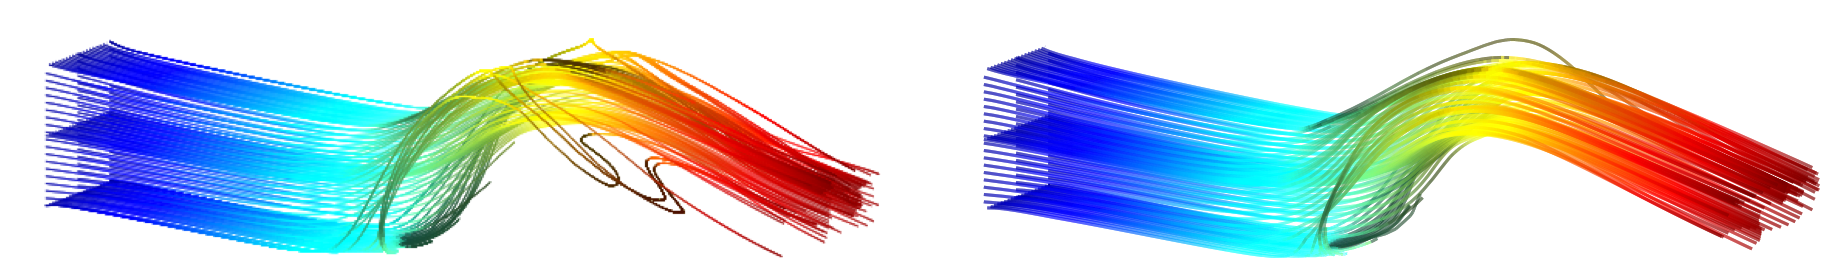
\includegraphics[width=\textwidth]{streamline2}
%  \end{center}
%  \includegraphics[height=\paperheight]{passat-front-right-crop}
}%
\begin{frame}[plain]
  %\titlepage
%\vfill
\leftline{\color{blue}\huge\bf Design optimisation}
\leftline{\color{blue}\huge\bf  for steady and unsteady flows}
\leftline{\color{blue}\huge\bf using adjoint methods}
\vfill\vfill
  \begin{center}
%    \includegraphics[width=\textwidth]{flowfield}\\
    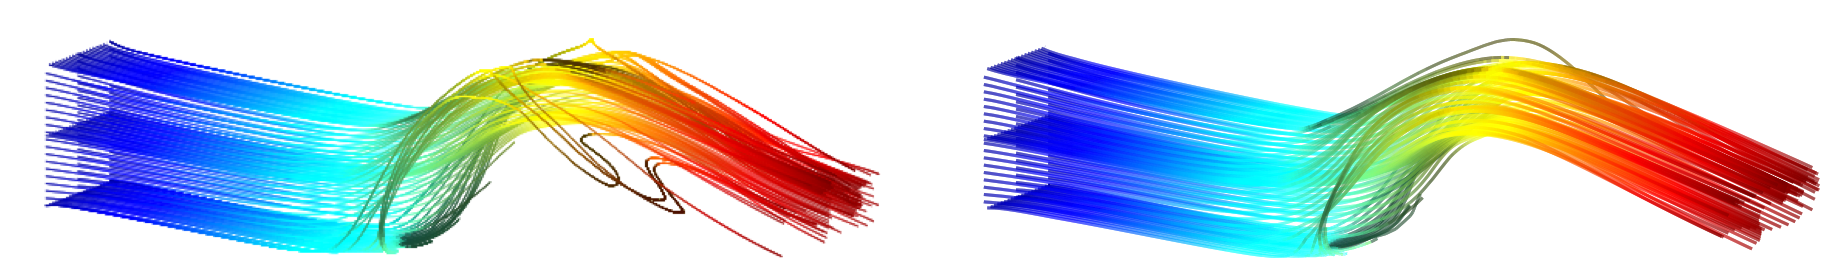
\includegraphics[width=\textwidth]{streamline2}
  \end{center}
\vfill\vfill

\leftline{\color{blue}\large\bf  Dr.~Jens-Dominik M\"{u}ller}
\leftline{\color{blue}\bf collaborators:}
\leftline{\color{blue}\bf 
          D.~Jones, F.~Christakpoulos, W.~Jahn, S.~Xu, M.~Oriani}
\leftline{\color{blue}\bf   {Queen Mary, University of London}}
\vfill

\begin{minipage}{\linewidth}
  \noindent
  \begin{minipage}[t]{.6\linewidth}
    \leftline{\color{blue} Fudan University, Shanghai, China}
    \leftline{\color{blue} 17 April 2013}
  \end{minipage} \hfil
  % \hspace{3 cm}
  \begin{flushright}
  
  \begin{minipage}{.3\linewidth}
%   \hspace{8cm}
   	  
\includegraphics[width=.3\linewidth]{logo_PW}
  \end{minipage}
  \end{flushright}
\end{minipage}
% \vfill
\end{frame}
\setbeamertemplate{background canvas}[default]

